\documentclass{article}
\usepackage{CJKutf8}
\usepackage{graphicx}
\usepackage{float}
\usepackage{listings}
\usepackage{multicol}
\usepackage{xcolor}
\graphicspath{ {../imgs/} }
\usepackage[pass]{geometry} % showframe is just for the example
\usepackage{hyperref}
\usepackage{kantlipsum} % just for the example




\begin{document}
\begin{CJK*}{UTF8}{gbsn}

\begin{titlepage}
\newgeometry{margin=3cm}
\centering

\vspace*{\stretch{2}}

\Large 搜索引擎爬虫与预处理

\vspace{\stretch{1}}

\normalsize The duration: 4 weeks
\vspace{\stretch{0.5}}

\begin{tabular}{ll}
Submission date & 2022.04.26 \\[2ex]
Student's name  & 陈浩楠 \\[2ex]
Student's ID & 2019112256\\[2ex]
From            & 计算机2019-01班
\end{tabular}

\vspace{\stretch{3}}


\vspace{\stretch{2}}
project location: 
\url{https://github.com/bianyuanop/search_engine_course_design}
\end{titlepage}

\tableofcontents
\pagebreak

\section{前言}
爬虫是搜索引擎的前置程序,用于收集网络中的网页数据,之后存储到本地做预处理。最后通过一系列算法的处理,可通过关键词使用户的到相关的页面。预处理作为搜索引擎的一个必要组成部分,在搜索结果的内容准确度上有着非常重要的作用。这样的预处理技术同样被应用于NLP领域,本项目采用Python作为主要开发语言,一方面考虑到Python作为一种胶水语言可以很好的组合不同的模块,加快开发速度;另一方面,因为Python在深度学习、人工智能领域的发展,其在相关领域的库和包非常丰富,减少了程序编写者的代码编写时间。例如在本项目中所使用的nltk(natural language toolkit),jieba(结巴)中的peddle-cut功能都收益于其发展。

\section{项目架构}
本项目采用自下而上的构架方法,逐步实现了爬虫、分词、数据库等模块,之后通过对单个模块进行测试,在保证一定程度上的可用性后,将各个模块组合起来,最后得到了一个自动的爬取-处理程序。在对整体性能、错误等进行一些修正后,最终得到最后的实际生产模块。
\begin{figure}[H]
\centering
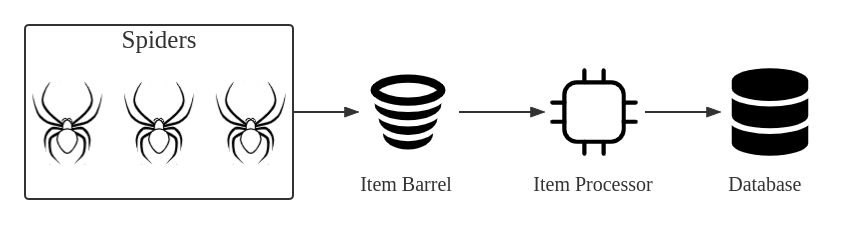
\includegraphics[height=3cm]{pipeline.png}
\caption{流水线}
\end{figure}
\subsection{Item Definition}
本项目使用了Scrapy作为基础Item的爬去器,在爬取到对应页面后,再通过流水线内的HTTP请求器请求对应页面获取HTML文本后再做处理。Item定义如下 ,
\begin{lstlisting}
class SpiderItem(scrapy.Item):
    base_site = scrapy.Field()
    title = scrapy.Field()
    href = scrapy.Field()
    url = scrapy.Field()
    filename = scrapy.Field()
    words_file = scrapy.Field()
\end{lstlisting}


\subsection{Processor}
\subsubsection{规范化}
Processor中则做两个操作,一个是规范化爬取后得到的链接,一般href中可以包含以下几类
\begin{itemize}
  \item //bilibili.com/av10492
  \item http://bilibili.com/cv1000
  \item https://bilibili.com/cv1
\end{itemize}
故需要将上述链接规范化为http开头或https开头的链接。如将
$//bilibili.com/av10492$ 转换为 $https://bilibili.com/av10492$
\subsubsection{文档处理}
对于不同的爬虫,采用不同的处理方法。如对于中文站,我们采取分词,再删除其停用词后再保存。而对于英文站,我们则需先获取词根,再删除停用词。最后再储存至文件,存储完成后在数据库中写入记录(网页文件名, url, 关键词文件名)。
\subsection{数据库}
按存储需要,数据库中只存储一张表,共四个字段。
\begin{lstlisting}
CREATE TABLE IF NOT EXISTS data
(
    id INTEGER PRIMARY KEY AUTOINCREMENT,
    filename TEXT,
    url TEXT,
    words_file TEXT
);
\end{lstlisting}
按操作需要,这里需要两条操作语句:
\begin{itemize}
	\item 查询某url是否已经被爬取过
	\item 插入记录
\end{itemize}
即:
\begin{lstlisting}
self.cursor.execute('''
INSERT INTO data (filename, url, words_file)
VALUES (?, ?, ?)
''', (item['filename'],item['url'], item['words_file']))
\end{lstlisting}
和
\begin{lstlisting}
cur = self.cursor.execute("SELECT * FROM data WHERE url = ?", (url,))
return cur.fetchone() is not None
\end{lstlisting}


\section{爬虫}
\qquad 网络爬虫(英语:web crawler),也叫网络蜘蛛(spider),是一种用来自动浏览万维网的网络机器人。其目的一般为编纂网络索引。网络搜索引擎等站点通过爬虫软件更新自身的网站内容或其对其他网站的索引。网络爬虫可以将自己所访问的页面保存下来,以便搜索引擎事后生成索引供用户搜索。爬虫访问网站的过程会消耗目标系统资源。不少网络系统并不默许爬虫工作。因此在访问大量页面时,爬虫需要考虑到规划、负载,还需要讲“礼貌”。 不愿意被爬虫访问、被爬虫主人知晓的公开站点可以使用robots.txt文件之类的方法避免访问。这个文件可以要求机器人只对网站的一部分进行索引,或完全不作处理。互联网上的页面极多,即使是最大的爬虫系统也无法做出完整的索引。因此在公元2000年之前的万维网出现初期,搜索引擎经常找不到多少相关结果。现在的搜索引擎在这方面已经进步很多,能够即刻给出高质量结果。\cite{crawler}

\begin{figure}[H]
\centering

\includegraphics[height=8cm]{WebCrawlerArchitecture.svg.png}
\caption{一般网络爬虫架构\cite{crawler}}
\end{figure}
在本项目中,则采用了Scrapy框架作为Spider的reactor,简单的编辑起始站点、解析函数则可得到一个同要架构的高性能爬虫。
\subsection{抓取}
\begin{figure}[H]
\centering
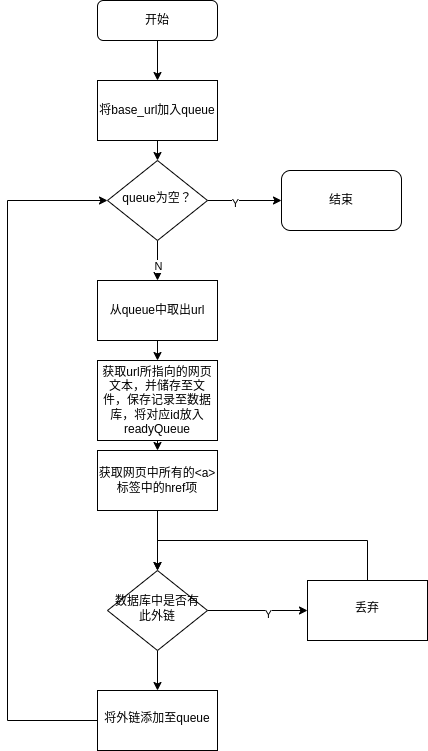
\includegraphics[width=8cm]{spider_flow.drawio.png}
\caption{爬取流程}
\end{figure}
在上述流程的每一步,Scrapy都会生成一个Item作为输入投入流水管线。在流水管线中采用了requests作为单个网页的抓取,简单的几行代码即可得到网页的信息,如:
\begin{lstlisting}
import requests
url = "someurl"
response = requests.get(url)
if response.ok:
	content = response.content 
\end{lstlisting}
\subsection{Scrapy}
Scrapy是一个开源、社区协作完成的爬虫框架,用于提取用户需要的特定数据。
\begin{figure}[H]
\centering
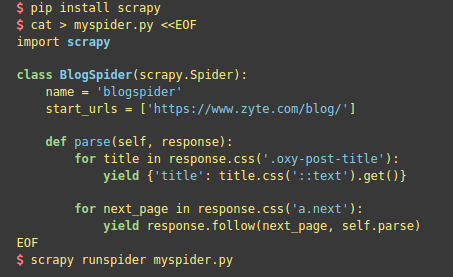
\includegraphics[width=10cm]{scrapy1.png}
\caption{示例Spider\cite{scrapy}}
\end{figure}
\begin{figure}[H]
\centering
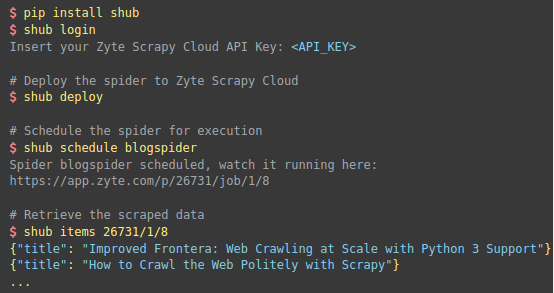
\includegraphics[width=10cm]{scrapy2.png}
\caption{运行\cite{scrapy}}
\end{figure}

\subsubsection{bilibili spider}
Bilibili,又称b站。本项目爬取的内容为b站在专栏推送的文章,在它的主页分析了一下xhr请求发现,它有着一个固定的api调用,且此api返回的结果每一次都是随机的。故使用此api返回的结果作为起始页开始爬取。
\begin{figure}[H]
\centering
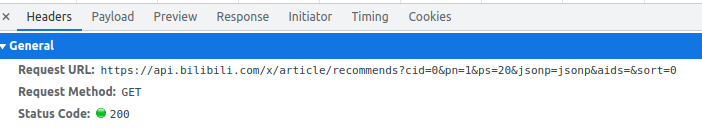
\includegraphics[width=14cm]{bili1.png}
\caption{Api请求}
\end{figure}
\begin{figure}[H]
\centering
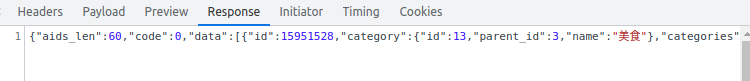
\includegraphics[width=14cm]{bili2.png}
\caption{JSON返回值}
\end{figure}

启动函数 $start\_requests$:
\begin{lstlisting}
start_api = 'https://api.bilibili.com/x/article/recommends\?cid\=0\&pn\=1\&ps\=20\&jsonp\=jsonp\&aids\=\&sort\=0' 
base_url = 'https://www.bilibili.com/read/cv'

stream = os.popen("curl https://api.bilibili.com/x/article/recommends\?cid\=0\&pn\=1\&ps\=20\&jsonp\=jsonp\&aids\=\&sort\=0")
jsonStr = stream.read()
jsonObj = json.loads(jsonStr)
pagesInfos = jsonObj['data']
for pageInfo in pagesInfos:
    link = base_url + str(pageInfo['id'])
    yield scrapy.Request(url=link, callback=self.parse)
\end{lstlisting}
解析函数$parse$:
\begin{lstlisting}
	items = SpiderItem()
        items['base_site'] = 'bilibili.com'

        for q in response.css('.article-item'):
            items['title'] = q.css('.article-title::text').get()
            items['href'] = q.css('a::attr("href")').get()

            yield items

        next_page = items.get('href')
        if next_page is not None and self.count < 10:
            yield response.follow(next_page, callback=self.parse)
\end{lstlisting}


\subsubsection{stackoverflow spider}
至于StackOverflow,则使用$https://stackoverflow.com/questions$此链接下的文章,以及使用最下的页脚作跳转。
启动链接 $start_urls$:
\begin{lstlisting}
start\_urls = [
        'https://stackoverflow.com/questions'
    ]
\end{lstlisting}
解析函数$parse$:
\begin{lstlisting}
items = SpiderItem()

for q in response.css('.s-post-summary--content-title'):
    items['base_site'] = 'stackoverflow.com'
    items['title'] = q.css('a::text').get() 
    items['href'] = q.css('a::attr("href")').get()

    yield items
        
next_page = response.css('.s-pagination--item.js-pagination-item[rel="next"] \
	::attr("href")').get()
if next_page is not None and self.count < 10:
    yield response.follow(next_page, callback=self.parse)
\end{lstlisting}



 
\subsection{网页解析}
\qquad 网页解析方面,使用了一个著名的Html解析库 - BeautifulSoup4,这个库提供了基本的html tag解析功能,在html文本输入后,可以生成一个soup对象,对于这个对象,我们可以对它进行遍历以获取所有标签链接,以及每个链接中的文本。对于外链的获取,一般而言,html中的外链一般使用tag名为a的标签包含外链。一般格式为$<a\ href="somelink">text\ description</a>$, 用css选择器的语法则可以这样提取:

\begin{lstlisting}
tags = document.querySelectorAll('a[href]')
// iterate tags and further disposing 
...
\end{lstlisting}
\begin{figure}[H]
\centering
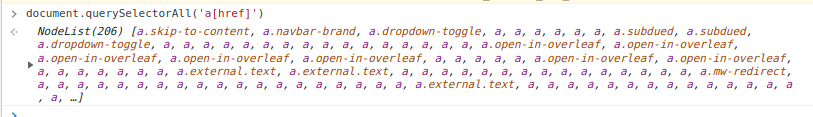
\includegraphics[height=2cm]{query_selector.png}
\caption{css选择题样例}
\end{figure}

而对于文本提取,则有以下两种情况:\newline
\begin{multicols}{2}
\color{blue}
情况一: 文本全位于叶节点
\color{black}
\begin{lstlisting}[
    basicstyle=\small, %or \small or \footnotesize etc.
]
<html>
<body>
<div>
  <a href="hello">hello</a>
  <a href="hello">another</a>
<div>
</body>
</html>
\end{lstlisting}

\columnbreak
\color{blue}
情况二: 部分文本位于父节点
\color{black}
\begin{lstlisting}[
    basicstyle=\small, %or \small or \footnotesize etc.
]
<html>
<body>
<div>
  <a href="hello">hello</a>
  <a href="hello">another</a>
  <!-- parent text -->
  parent text
<div>
</body>
</html>
\end{lstlisting}
\end{multicols}
在BeautifulSoup\cite{soup}中,一个节点的文本信息可以用 $.string$ 获取,但是这种情况只在叶节点有效,如果节点为父节点,那么这个方法将会将字节点的raw content作为输出。所以通常我们只在叶节点调用这个方法。但这样的方法在第二种情况会导致信息丢失。故我们需要在遍历时,在取出叶节点文本后,将叶节点删除,最后使它的父节点退化成叶节点已进行操作。\newline\newline
两种方法分别对情况二中的文本进行处理后的结果分别为:\newline
\begin{table}[H]
\begin{tabular}{lllll}
\cline{1-2}
\multicolumn{1}{|l|}{BFS}           & \multicolumn{1}{l|}{BFS with deletion}         &  &  &  \\ \cline{1-2}
\multicolumn{1}{|l|}{hello another} & \multicolumn{1}{l|}{hello another parent text} &  &  &  \\ \cline{1-2}
                                    &                                                &  &  &  \\
                                    &                                                &  &  & 
\end{tabular}
\end{table}
伪代码如下:
\begin{lstlisting}
FUNC GET_TEXT(node)
	IF node is leaf:
		APPEND node.content
	ELSE:
		FOR child in node:
			GET_TEXT(child)
			DELETE child
		APPEND node.content
ENDFUNC
\end{lstlisting}


\section{预处理}

预处理的流程为
\begin{table}[H]
\begin{tabular}{ll}
  & Step  \\
1 & 分词    \\
2 & 删除重复词 \\
3 & 删除停用词 \\
4 & 生成词根  \\
  &      
\end{tabular}
\end{table}
\subsection{停用词}
\qquad Stopwords ISO 中的英文和中文听用词表:

\begin{figure}[H]
\centering
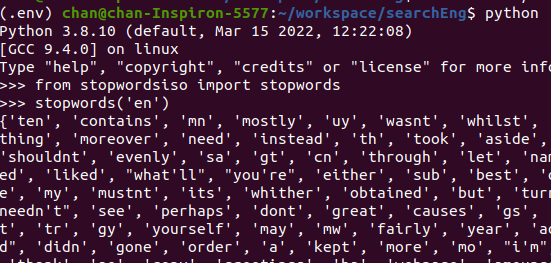
\includegraphics[height=5cm]{stopwords_en.png}
\caption{en stopwords}
\end{figure}

\begin{figure}[H]
\centering
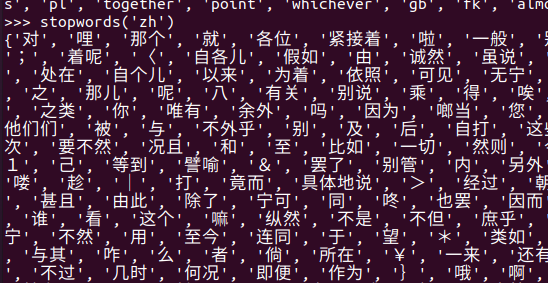
\includegraphics[height=5cm]{stopwords_zh.png}
\caption{zh stopwords}
\end{figure}
\subsection{分词}
\subsubsection{中文分词}
\qquad 中文分词使用了Python中的jieba\cite{jieba}库,jieba支持一下几种模式
\begin{itemize}
  \item 精确模式,试图将句子最精确地切开,适合文本分析。
  \item 全模式,把句子中所有的可以成词的词语都扫描出来, 速度非常快,但是不能解决歧义。
  \item 搜索引擎模式,在精确模式的基础上,对长词再次切分,提高召回率,适合用于搜索引擎分词。
  \item paddle模式,利用PaddlePaddle深度学习框架,训练序列标注(双向GRU)网络模型实现分词。同时支持词性标注。
\end{itemize}
一个样例输入:\newline
\qquad 维基百科最早是在吉米·威尔士与拉里·桑格两人的合作下于2001年1月13日在互联网上推出的网站服务,并于1月15日正式展开网络百科全书项目。其中桑格结合了维基百科网站合作核心之“Wiki”以及具有百科全书之意的“encyclopedia”创造出新混成词“Wikipedia”。在创立之初,维基百科的目标是向全人类提供自由的百科全书,并希望各地民众能够使用自己选择的语言来参与编辑条目。其他书面印刷的百科全书多是由专家主导编辑,之后再由出版商印刷并加以销售。维基百科在性质上一如其号称般属于可自由访问和编辑的全球知识体,这也意味着除传统百科全书所收录的信息外,维基百科也能够收录非学术但仍具有一定媒体关注度的动态事件。2006年《时代》杂志所评选的时代年度风云人物“你”中,便提到了全球上百万人于线上以协作方式促进了维基百科的快速成长,同年提及的其他重要网站还有YouTube、MySpace和Facebook。
来自 \url{https://zh.wikipedia.org/wiki/%E7%BB%B4%E5%9F%BA%E7%99%BE%E7%A7%91}
\newline
分词输出:\newline
\begin{figure}[H]
\centering

\includegraphics[height=5cm]{cut_words_cn.png}
\caption{中文分词样例}
\end{figure}
\subsubsection{英文词根生成}
样例输入:\newline
NLTK is a leading platform for building Python programs to work with human language data. It provides easy-to-use interfaces to over 50 corpora and lexical resources such as WordNet, along with a suite of text processing libraries for classification, tokenization, stemming, tagging, parsing, and semantic reasoning, wrappers for industrial-strength NLP libraries, and an active discussion forum.
来自\url{https://www.nltk.org/}
\newline
样例输出:\newline
\begin{figure}[H]
\centering
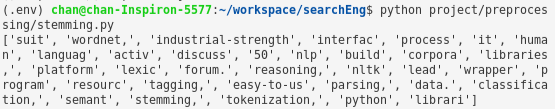
\includegraphics[height=3cm]{en_stem_result.png}
\caption{词根生成}
\end{figure}

\section{结果}
\begin{figure}[H]
\centering
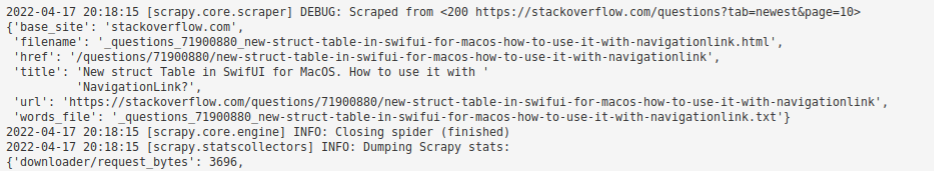
\includegraphics[height=3cm]{result.png}
\caption{主程序运行时}
\end{figure}

\begin{figure}[H]
\centering
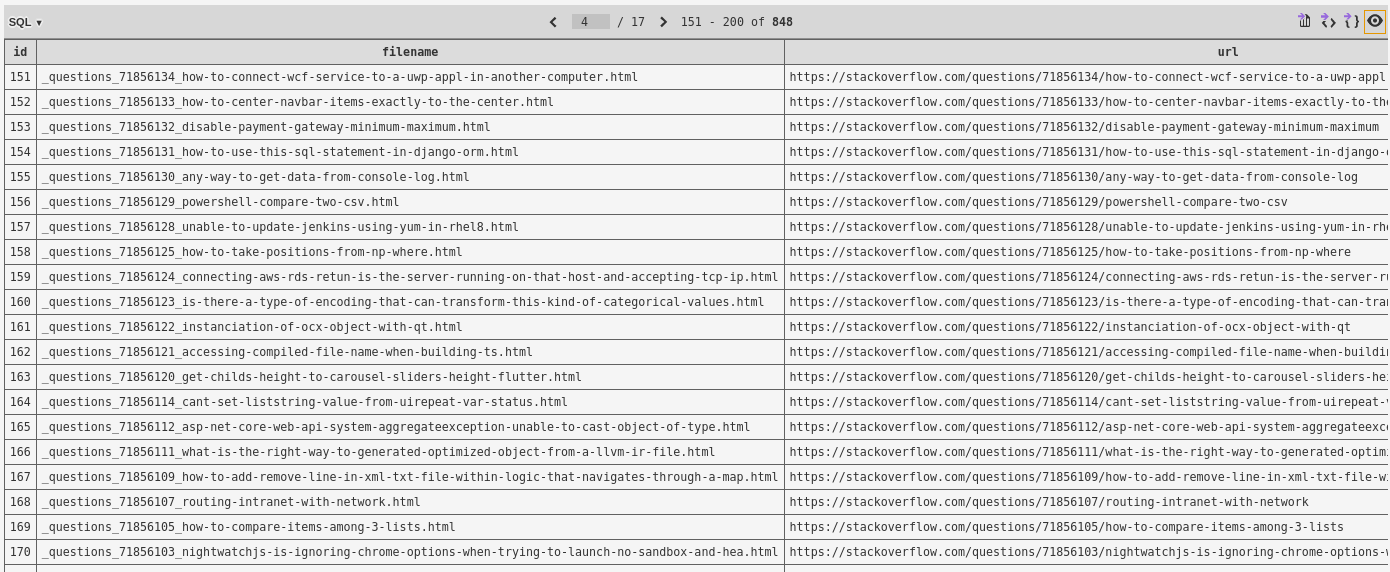
\includegraphics[height=6cm]{query_result.png}
\caption{数据记录}
\end{figure}

\begin{figure}[H]
\centering
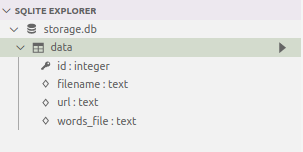
\includegraphics[height=4cm]{db_table.png}
\caption{数据表}
\end{figure}

\begin{figure}[H]
\centering
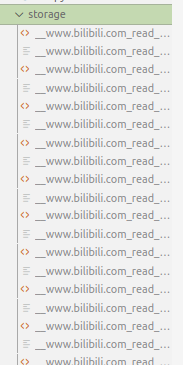
\includegraphics[height=10cm]{storage.png}
\caption{储存文件夹}
\end{figure}


\newpage
\begin{thebibliography}{}
\bibitem{crawler}
网络爬虫. (2022). In 维基百科,自由的百科全书. https://zh.wikipedia.org/w/index.php?title=网络爬虫
\bibitem{jieba}
Junyi, S. (2022). Jieba [Python]. https://github.com/fxsjy/jieba (Original work published 2012)
\bibitem{soup}
Beautiful Soup Documentation—Beautiful Soup 4.4.0 documentation. (n.d.). Retrieved March 30, 2022, from https://beautiful-soup-4.readthedocs.io/en/latest/
\bibitem{nltk}
NLTK :: Natural Language Toolkit. (n.d.). Retrieved March 30, 2022, from https://www.nltk.org/
\bibitem{stopwordsiso}
Stopwords ISO. (2022). [JavaScript]. Stopwords ISO. https://github.com/stopwords-iso/stopwords-iso (Original work published 2016)
\bibitem{scrapy}
Scrapy | A Fast and Powerful Scraping and Web Crawling Framework. (不详). 取读于 2022年4月17日, 从 https://scrapy.org/



\end{thebibliography}

\end{CJK*}
\end{document}